\section{Umsetzung}
%was für komponenten braucht, etwas was auffinden ermöglicht, etwas was als server fungiert, jeder client ist server und client, wie finde ich server
%Erst erklären was ich machen: wie hab ich es gemacht. Hier auch diagramme einfügen 
Im Rahmen dieser Arbeit wird eine peer-to-peer Chat-Anwendung entwickelt mit der Verwendung von Client-Server Technologie.
Um einen funktionierenden Chatroom zu bauen werden verschiedene Komponenten für verschiedene Aufgaben benötigt. 
Der Chat client setzt sich im wesentlichen zusammen aus:
\begin{itemize}
    \item Receiver
    \item Transmitter
    \item DiscoveryService
    \item ConfigData
    \item Message types
\end{itemize} 
Beim Starten der Chat-Anwendung findet eine Initialisierung statt. Der Client soll mithilfe eines mdns Broadcast andere Chatteilnehmer finden.
Wurde ein anderer Teilnehmer gefunden bekommt der Client eine mdns Antwort mit der IP Adresse des Teilnehmers.
Die IP Adresse wird in eine Userliste eingetragen. 
An jede gedundene IP Adresse wird eine Startmessage mit eigener IP Adresse und Name über HTTP geschickt. Der andere Teilnehmer kann somit den neuen 
User in seiner Liste ergänzen und ebenfalls eine Startmessage mit seinem Namen als Antwort schicken. Der neue Client ergänzt in seiner Userliste 
den Namen. Damit ist die Initialisierung abgeschlossen. 
\begin{figure}[ht]
    \centering
    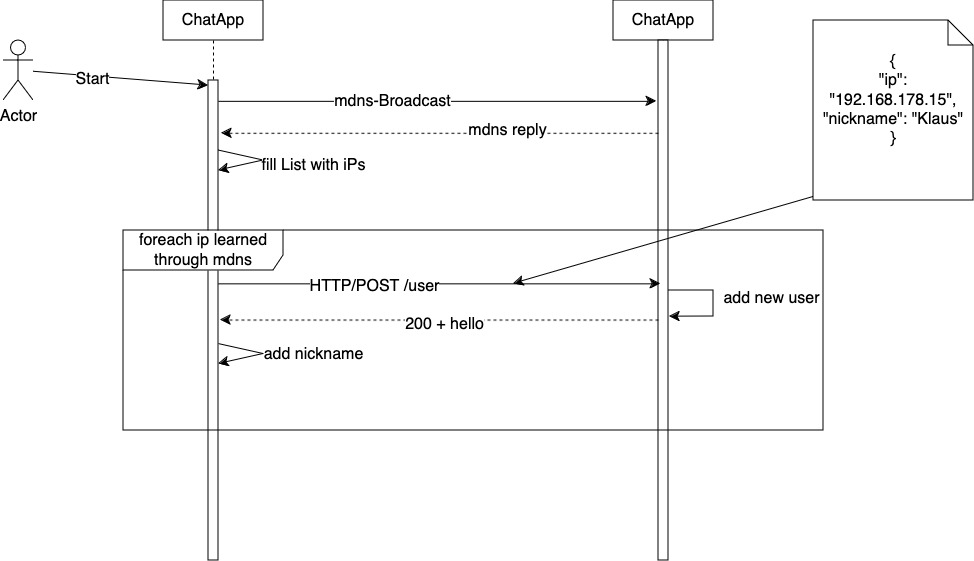
\includegraphics[scale=0.4]{Images/Initialisierung_Sequenzdiagramm.jpg}
    \captionbelow{Initialisierung}
\end{figure}
\\
\\
Nachdem man dem Chatroom beigetreten ist können Nachrichten verschickt werden. Der User schreibt eine Nachricht. 
Um diese Nachricht zu verschicken muss der Client in der Userliste alle IP Adressen der Teilnehmer nachschauen. Die Nachricht wird anschließend 
an jede einzelne IP Adresse geschickt. Das Versenden der Nachrichten findet ebenfalls mittels HTTP statt.
\begin{figure}[ht]
    \centering
    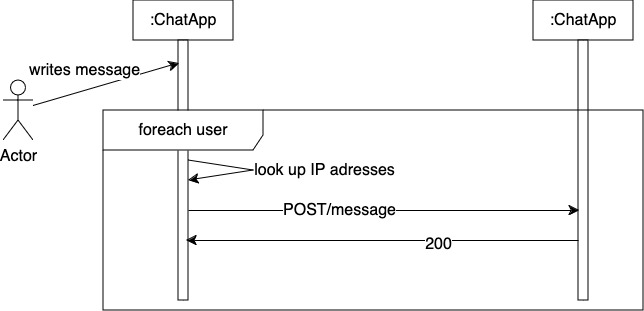
\includegraphics[scale=0.4]{Images/Conversation_Sequenzdiagramm.jpg}
    \captionbelow{Kommunikation}
\end{figure}
\\
\\
Um den Chatroom zu verlassen wird wieder über HTTP eine Exitmessage an alle Teilnehmer gesendet. Die Exitmessage enthält wie die Startmessage den eigenen Namen und IP Adresse.
Der User wird von den anderen Teilnehmern aus der Userliste entfernt und der Client ist somit dem Chatroom ausgetreten. 
\begin{figure}[ht]
    \centering
    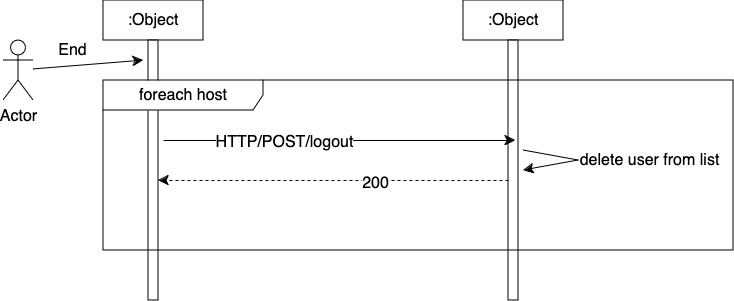
\includegraphics[scale=0.4]{Images/Exit_Sequenzdiagramm.jpg}
    \captionbelow{Exit}
\end{figure}






%Beim Starten des Chat clients sucht der DiscoveryService mithilfe eines Multicasts nach anderen Benutzern.
%Alle Nachrichten werden über eine REST API an den richtigen Endpunkt geschickt. Es gibt drei verschiedene Endpunkte: Start, Message, Exit.
%Es wird eine Startmessage mit eigenem Namen und IP Adresse an die IP Adresse des gefundenen Teilnehmers geschickt.  
%Die IP Adresse wird in der Userliste der Configdata eingetragen.
%Der Receiver nimmt die Antwort auf die Startmessage entgegen. Diese enthält den Namen des gefundenen Teilnehmers, sodass er passend zur IP Adresse in der Userliste ergänzt werden kann.
%Jeder neue Teilnehmer tritt über den beschriebenen Startprozess dem Chatroom bei. 

%Der Transmitter ist für das Senden von Nachrichten zuständig. In der Userliste werden die IP Adressen der Teilnehmer nachgeschaut. 
%Die Nachricht wird an den Endpunkt Message und somit an jede einzelne IP Adresse der Liste geschickt. 

%Verlässt ein Teilnehmer den Chatroom, wird eine Exitmessage an den Endpunkt Exit geschickt. Die Exitmessage wird vom Receiver entgegen genommen. 
%Hierbei wird der Name und die IP Adresse gesendet um aus der Userliste gelöscht zu werden. 
%Es wird eine REST API für das Versenden von Nachrichten verwendet